\documentclass[a4paper,12pt]{article}
\usepackage[utf8]{inputenc}

\usepackage[utf8]{inputenc}
\usepackage[T2A]{fontenc}
\usepackage[english,russian]{babel}
\usepackage{amsthm}
\usepackage{amsmath}
\usepackage{amssymb}
\usepackage{tikz}
\usepackage{textcomp}
\usepackage{marvosym}
\usepackage{ esint }
\usepackage{mathtext}
\usepackage{siunitx} % Required for alignment
\usepackage{subfigure}
\usepackage{multirow}
\usepackage{rotating}
\usepackage{afterpage}
\usepackage[arrowdel]{physics}
\usepackage{booktabs}
\setlength{\topmargin}{-0.5in}
\setlength{\textheight}{9.1in}
\setlength{\oddsidemargin}{-0.4in}
\setlength{\evensidemargin}{-0.4in}
\setlength{\textwidth}{7in}
\setlength{\parindent}{0ex}
\setlength{\parskip}{1ex}
\newcommand{\ndiv}{\hspace{-4pt}\not|\hspace{2pt}}
\usepackage{graphicx}
\usepackage{float}
\usepackage{wrapfig}
\usepackage{pgfplots}
\usepackage{caption}
\pgfplotsset{compat=1.16}
\graphicspath{ {./images/} }
\usepackage{graphicx}
\RequirePackage{caption}
\DeclareCaptionLabelSeparator{defffis}{ — }
\captionsetup{justification=centering,labelsep=defffis}
\usepackage{caption} \captionsetup[table]{labelsep=endash,justification=justified,singlelinecheck=false,font=normalsize}
\usepackage{amsfonts,mathtools}

\title{Лабораторная работа № 4.7.2\\Эффект Поккельса}
\author{Илья Прамский}
\date{Апрель 2024}

\begin{document}
\maketitle
\newpage

\textbf{Цель:} исследовать интерференцию рассеянного света, прошедшего кристалл; наблюдать изменение характера поляризации света при наложении на кристалл электрического поля.

\textbf{Оборудование:} гелий-неоновый лазер, поляризатор, кристалл ниобата лития, матовая пластинка, экран, источник высоковольтного переменного и постоянного напряжения, фотодиод, осциллограф, линейка.

\section{Теоретические сведения}
Эффект Поккельса -- изменение показателя преломления света в кристалле под действием электрического поля.

Рассмотрим кристалл ниобата лития $\text{LiNbO}_3$ с цетральноосевой симметрией вдоль оси $Z$. Для световой волны с $\mathbf{E}$ перпендикулярно $Z$ показатель преломления будет $n_o$, а для волны с $\mathbf{E}$ вдоль $Z$ -- $n_e$. В случае, когда луч света идёт под углом $\theta$ к оси, есть два значение показателя преломления $n_1$ и $n_2$: $n_1 = n_o$ для волны с $\mathbf{E}$ перпендикулярным плоскости $(\mathbf{k},\mathbf{Z})$ (обыкновенная волна) и $n_2$ для волны с $\mathbf{E}$ в этой плоскости (необыкновенная волна). В последнем случае
\begin{equation}
\dfrac{1}{n_2^2}=\dfrac{\cos^2 \theta}{n_0^2}+\dfrac{\sin^2 \theta}{n_e^2}.
\end{equation}

\begin{figure}[h]
	\center{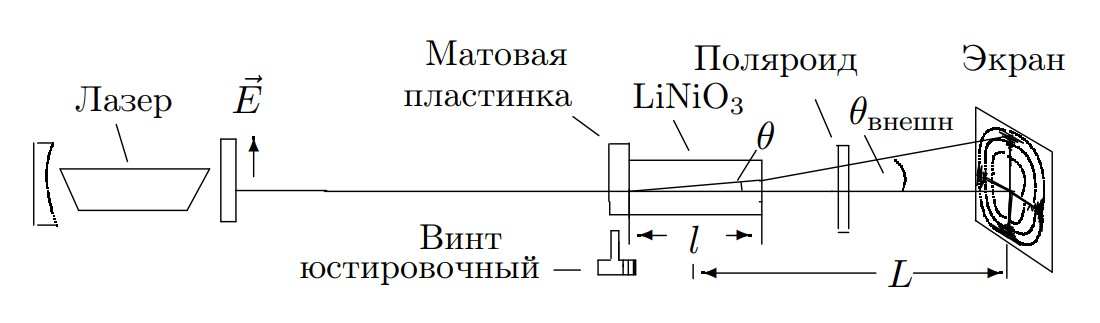
\includegraphics[scale=0.5]{1.jpg}}
  \caption{\centering Оптическая часть экспериментальной установки}
	\label{fig:image1}
\end{figure}

Если перед кристаллом, помещённым между поляроидами, расположить линзу или матовую пластинку, то на экране за поляроидом мы увидим тёмные концентрические окружности -- результат интерференции обыкновенной и необыкновенной волн. При повороте выходного поляроида на $90^\circ$ картина меняется с позитива на негатив (на месте светлых пятен появляются тёмные и наоборот). В случае, когда разрешённое направление анализатора перпендикулярно поляризации лазерного излучения, радиус тёмного кольца с номером $m$ равен
\begin{equation}
r_m^2 = \dfrac{\lambda}{l} \dfrac{(n_oL)^2}{n_0 - n_e}m,
\end{equation}

\begin{figure}[h]
	\center{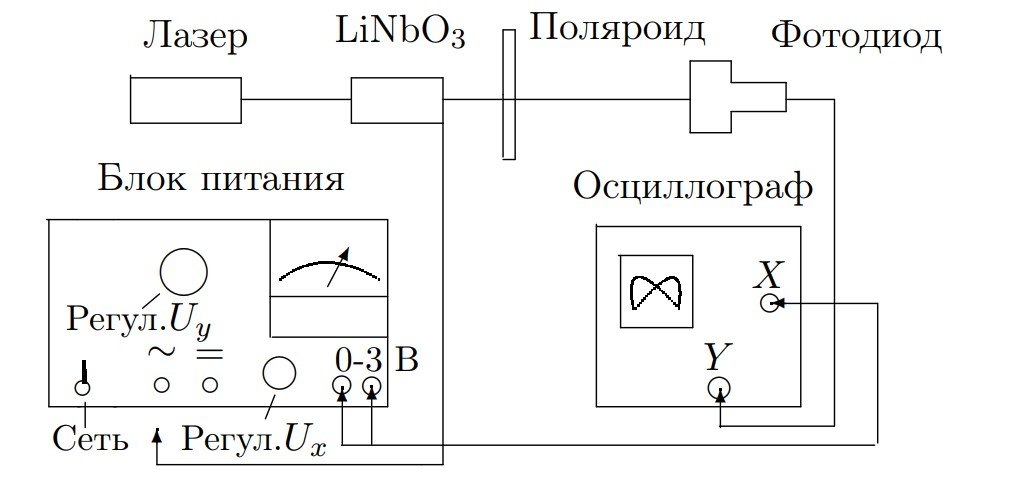
\includegraphics[scale=0.5]{2.jpg}}
 \caption{\centering Экспериментальная установка}
	\label{fig:image1}
\end{figure}

где $L$ -- расстояние от центра кристалла до экрана, $l$ -- длина кристалла.

Теперь поместим кристалл в постоянное электрическое поле $E_{\text{эл}}$, направленное вдоль оси $X$, перпендикулярной $Z$. Показатель преломления для луча, распространяющего вдоль $Z$, всегда $n_o$. В плоскости $(X,Y)$ возникают два главных направления под углами $45^\circ$ к $X$ и $Y$ с показателями преломления $n_0 - \Delta n$ и $n_o + \Delta n$ (быстрая и медленная ось), причём $\Delta n = A E_{\text{эл}}$. Для поляризованного вертикально света и анализатора, пропускающего горизонтальную поляризацию, на выходе интенсивность на выходе будет иметь вид
\begin{equation}
I_{\text{вых}} = I_0 \sin^2 \left(\dfrac{\pi}{2} \dfrac{U}{U_{\lambda/2}} \right),
\end{equation}
где $\displaystyle U_{\lambda/2} = \frac{\lambda}{4A}\frac{d}{l}$ -- \textit{полуволновое напряжение}, $d$ -- поперечный размер кристалла.  При напряжении $U = E_{\text{эл}}d$ равном полуволновому сдвиг фаз между двумя волнами равен $\pi$, а интенсивность света на выходе максимальна. 


На Рис. 2 представлена схема всей установки (оптическая часть изорбажена на Рис. 1). Свет лазера, проходя через сквозь пластину, рассеивается и падает на двоякопреломляющий кристалл. На экране за поляроидом видна интерференционная картина. Убрав рассеивающую пластину и подавая на кристалл постоянное напряжение, можно величиной напряжения влиять на поляризацию луча, вышедшего из кристалла. Заменив экран фотодиодом и подав на кристалл переменное напряжение, можно исследовать поляризацию с помощью осциллографа.
\section{Ход работы}
Для начала проведём юстировку системы. Соберём оптическую схему. Включим лазер и установим анализатор (без кристалла в схеме) так, чтобы лазерное излучение через него не проходило (скрещенные поляризации). Поставим кристалл и установим перед ним вплотную к кювете матовую пластинку. Выпишем также её параметры, которые в дальнейшем понадобятся для расчётов. $\lambda = 0,63$ мкм, $n_o = 2,29$, $l = 26$ мм, $L = 77,5 \pm 0,5$ см.

Получим на экране интерференционную картину.

\begin{figure}[H]
	\centering
	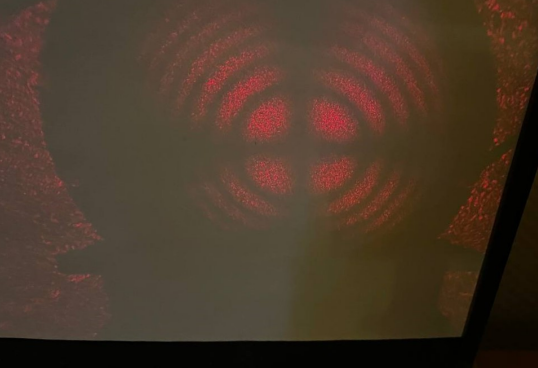
\includegraphics[scale=1]{photo1.png}
\end{figure}

Теперь измерим радиусы тёмных колец и занесём данные в таблицу. По этим данным построим график зависимости $r^2 = f(m)$, а затем при помощи угла наклона по формуле $(2)$ определим двулучепреломление $n_o - n_e$.

\begin{table}[H]
	\centering
	\begin{tabular}{|c|c|c|}
		\hline
		m & r, см & $r^2, \text{см}^2$ \\ \hline
		1 & 2,9 & 8,41 \\ \hline
		2 & 4,1 & 16,81 \\ \hline
		3 & 5,0 & 25,00 \\ \hline
		4 & 5,7 & 32,49 \\ \hline
		5 & 6,4 & 40,96 \\ \hline
		6 & 7,0 & 49,00 \\ \hline
		7 & 7,5 & 56,25 \\ \hline
		8 & 8,0 & 64,00 \\ \hline
	\end{tabular}
\end{table}

\begin{figure}[H]
	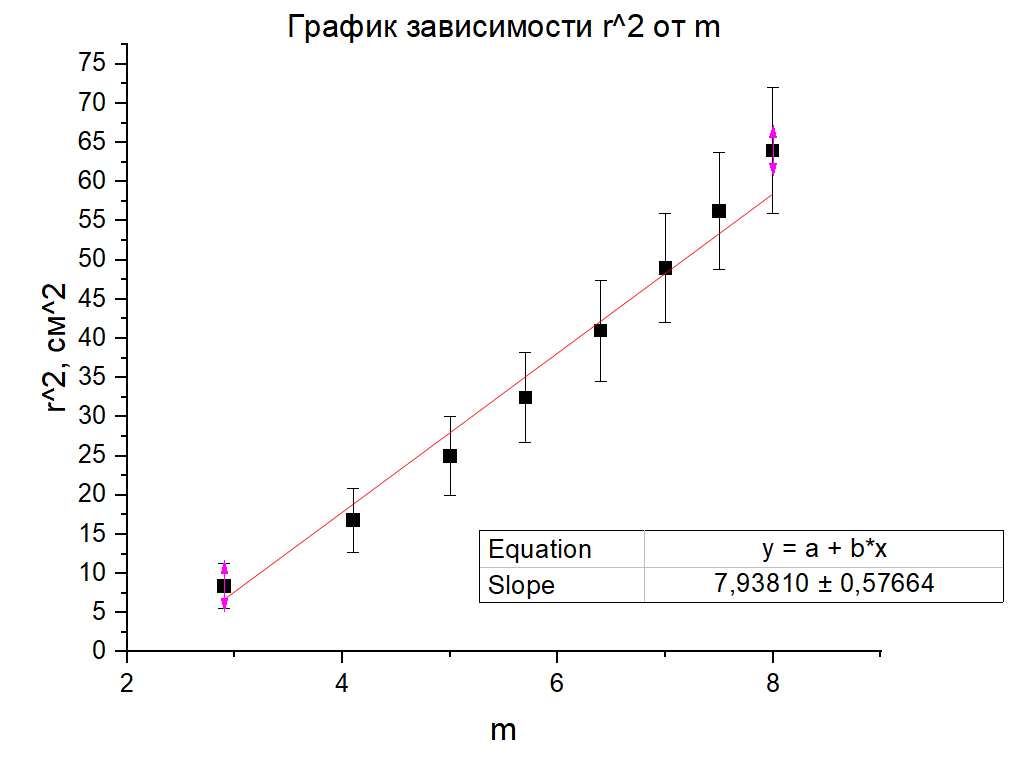
\includegraphics[scale=0.8]{graph1.png}
\end{figure}

Из графика $k = 7,9 \pm 0,6$. Тогда
\[n_o - n_e = \frac{\lambda {(n_oL)}^2}{lk} = 0,097 \pm 0,007\]
Табличное же значение равно 0,09, данное значение входит в диапазон погрешности.

Теперь перейдём ко второй части эксперимента. 
Подключим разъём блока питания на постоянное напряжение, установим регулятор напряжения на минимальное напряжение и включим блок питания в сеть.

С увеличением напряжения на кристалле яркость пятна на экране увеличивается и достигает максимума при $U = U_{\frac{\lambda}{2}} = 480 \pm 15$ В.

Также проверим, что при $U_\lambda = 960 \pm 30$ В, пятно имеет минимальную яркость.

При изменении поляризации на параллельную, $U_{\frac{\lambda}{2}} =  885 \pm 15$ В.

Также, подав напряжение, равное $U_{\frac{\lambda}{4}} = 240 \pm 8$ В, заметим, что поляризация станет круговой(яркость при вращении поляроида никак не меняется).

Теперь включим осциллограф, поставим приёмник, и будем передавать на осциллограф по оси x напряжение, а по оси y интенсивность излучения на экране. Получаются фигуры Лиссажу.

\begin{figure}[H]
	\centering
	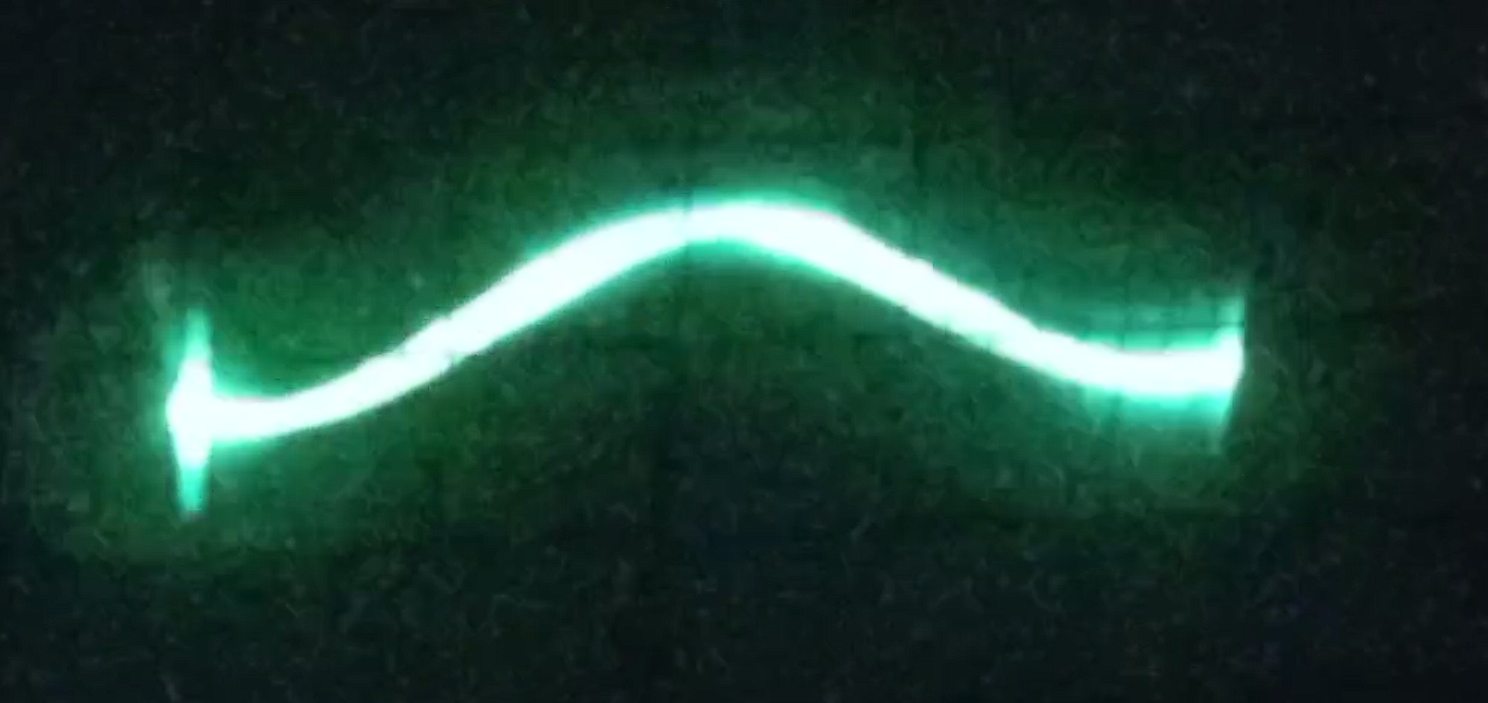
\includegraphics[scale=0.5]{photo2.png}
	\caption{Фигура Лиссажу при $U_{\frac{\lambda}{2}}$}
\end{figure}

\begin{figure}[H]
	\centering
	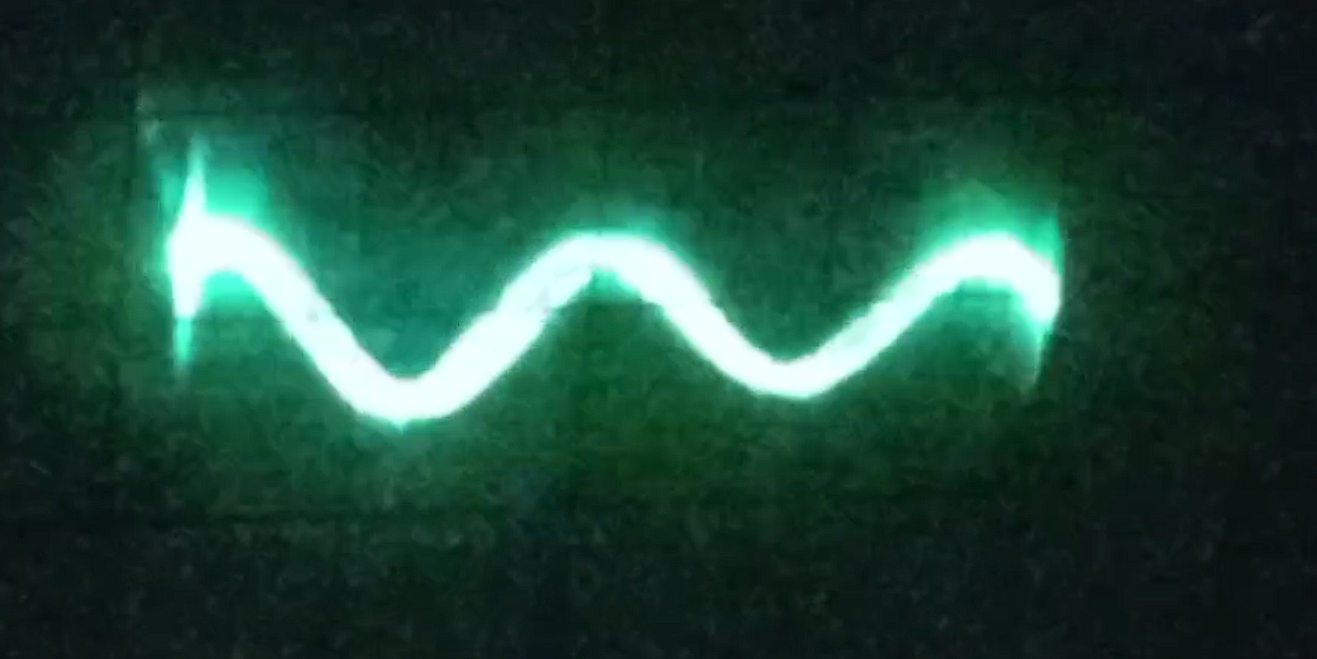
\includegraphics[scale=0.5]{photo3.png}
	\caption{Фигура Лиссажу при $U_{\lambda}$}
\end{figure}

\begin{figure}[H]
	\centering
	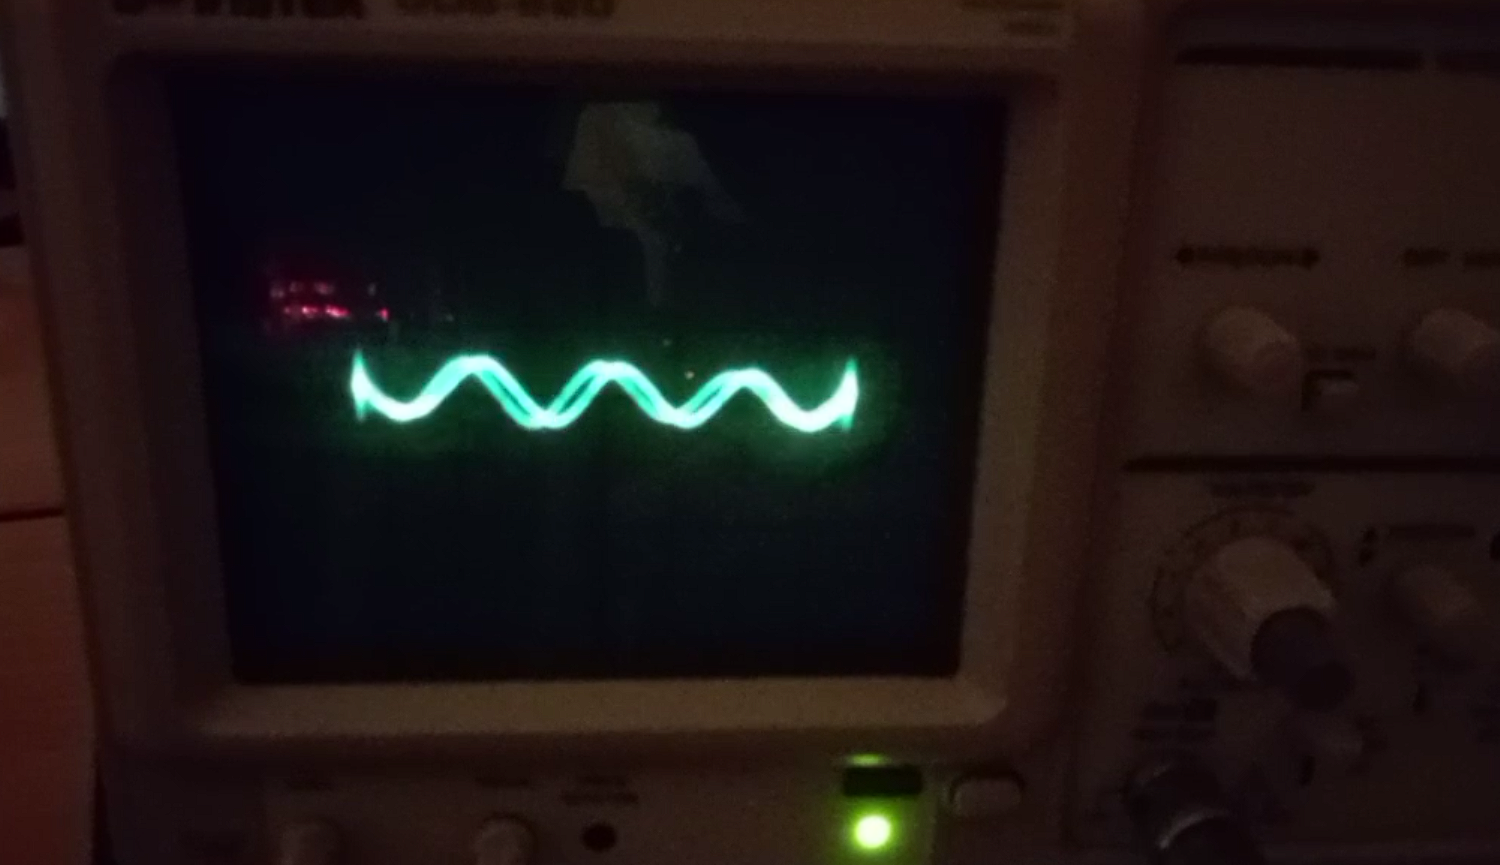
\includegraphics[scale=0.5]{photo4.png}
	\caption{Фигура Лиссажу при $U_{\frac{3\lambda}{2}}$}
\end{figure}

Найдём $U_{\frac{\lambda}{2}}$, как $\Delta U$, соответствующее переходу от максимума к минимуму сигнала. Получилось $\Delta U = 510 \pm 15$ В, что находится достаточно близко к полученному ранее значению.

\section{Вывод}
В ходе данной работы была исследована интерференция рассеяного света, прошедшего сигнал. Также при помощи исследования зависимости радиуса тёмного кольца от его номера, было вычислено двулучепреломление кристалла, равное $n_o - n_e = 0,097 \pm 0,007$ В, что находится достаточно близко к табличному значению(0,09 В). Также двумя различными способами было найдено значение напряжения, при котором яркость пятна достигает максимума, причём эти оба значения находятся близко друг к другу(480 и 510).

\begin{figure}
\centering
\includegraphics[scale=0.4]{photo5.jpg}
\caption{Я с коллегой(я слева, мой напарник - Денис Михайлов - справа}
\end{figure}
\end{document}